% Template for Elsevier CRC journal article
% version 1.2 dated 09 May 2011

% This file (c) 2009-2011 Elsevier Ltd.  Modifications may be freely made,
% provided the edited file is saved under a different name

% This file contains modifications for Procedia Engineering

% Changes since version 1.1
% - added "procedia" option compliant with ecrc.sty version 1.2a
%   (makes the layout approximately the same as the Word CRC template)
% - added example for generating copyright line in abstract

%-----------------------------------------------------------------------------------

%% This template uses the elsarticle.cls document class and the extension package ecrc.sty
%% For full documentation on usage of elsarticle.cls, consult the documentation "elsdoc.pdf"
%% Further resources available at http://www.elsevier.com/latex

%-----------------------------------------------------------------------------------

%%%%%%%%%%%%%%%%%%%%%%%%%%%%%%%%%%%%%%%%%%%%%%%%%%%%%%%%%%%%%%
%%%%%%%%%%%%%%%%%%%%%%%%%%%%%%%%%%%%%%%%%%%%%%%%%%%%%%%%%%%%%%
%%                                                          %%
%% Important note on usage                                  %%
%% -----------------------                                  %%
%% This file should normally be compiled with PDFLaTeX      %%
%% Using standard LaTeX should work but may produce clashes %%
%%                                                          %%
%%%%%%%%%%%%%%%%%%%%%%%%%%%%%%%%%%%%%%%%%%%%%%%%%%%%%%%%%%%%%%
%%%%%%%%%%%%%%%%%%%%%%%%%%%%%%%%%%%%%%%%%%%%%%%%%%%%%%%%%%%%%%

%% The '3p' and 'times' class options of elsarticle are used for Elsevier CRC
%% The 'procedia' option causes ecrc to approximate to the Word template
\documentclass[3p,times,procedia,number]{elsarticle}
\flushbottom

\usepackage{color}
\usepackage{subcaption}

%% The `ecrc' package must be called to make the CRC functionality available
\usepackage{ecrc}
\usepackage{amsmath}

\DeclareMathOperator*{\argmax}{arg\,max}

%% The ecrc package defines commands needed for running heads and logos.
%% For running heads, you can set the journal name, the volume, the starting page and the authors

%% set the volume if you know. Otherwise `00'
\volume{00}

%% set the starting page if not 1
\firstpage{1}

%% Give the name of the journal
\journalname{Procedia Engineering}

%% Give the author list to appear in the running head
%% Example \runauth{C.V. Radhakrishnan et al.}
\runauth{UGAWG}

%% The choice of journal logo is determined by the \jid and \jnltitlelogo commands.
%% A user-supplied logo with the name <\jid>logo.pdf will be inserted if present.
%% e.g. if \jid{yspmi} the system will look for a file yspmilogo.pdf
%% Otherwise the content of \jnltitlelogo will be set between horizontal lines as a default logo

%% Give the abbreviation of the Journal.
\jid{proeng}

%% Give a short journal name for the dummy logo (if needed)
%\jnltitlelogo{Procedia Engineering}

%% Hereafter the template follows `elsarticle'.
%% For more details see the existing template files elsarticle-template-harv.tex and elsarticle-template-num.tex.

%% Elsevier CRC generally uses a numbered reference style
%% For this, the conventions of elsarticle-template-num.tex should be followed (included below)
%% If using BibTeX, use the style file elsarticle-num.bst

%% End of ecrc-specific commands
%%%%%%%%%%%%%%%%%%%%%%%%%%%%%%%%%%%%%%%%%%%%%%%%%%%%%%%%%%%%%%%%%%%%%%%%%%

%% The amssymb package provides various useful mathematical symbols

\usepackage{amssymb}
%% The amsthm package provides extended theorem environments
%% \usepackage{amsthm}

%% The lineno packages adds line numbers. Start line numbering with
%% \begin{linenumbers}, end it with \end{linenumbers}. Or switch it on
%% for the whole article with \linenumbers after \end{frontmatter}.
%% \usepackage{lineno}

%% natbib.sty is loaded by default. However, natbib options can be
%% provided with \biboptions{...} command. Following options are
%% valid:

%%   round  -  round parentheses are used (default)
%%   square -  square brackets are used   [option]
%%   curly  -  curly braces are used      {option}
%%   angle  -  angle brackets are used    <option>
%%   semicolon  -  multiple citations separated by semi-colon
%%   colon  - same as semicolon, an earlier confusion
%%   comma  -  separated by comma
%%   numbers-  selects numerical citations
%%   super  -  numerical citations as superscripts
%%   sort   -  sorts multiple citations according to order in ref. list
%%   sort&compress   -  like sort, but also compresses numerical citations
%%   compress - compresses without sorting
%%
%\biboptions{authoryear}

 \biboptions{sort&compress}

% if you have landscape tables
\usepackage[figuresright]{rotating}
%\usepackage{harvard}
% put your own definitions here:x
%   \newcommand{\cZ}{\cal{Z}}
%   \newtheorem{def}{Definition}[section]
%   ...

% add words to TeX's hyphenation exception list
%\hyphenation{author another created financial paper re-commend-ed Post-Script}

% declarations for front matter

\begin{document}

\begin{frontmatter}

%% Title, authors and addresses

%% use the tnoteref command within \title for footnotes;
%% use the tnotetext command for the associated footnote;
%% use the fnref command within \author or \address for footnotes;
%% use the fntext command for the associated footnote;
%% use the corref command within \author for corresponding author footnotes;
%% use the cortext command for the associated footnote;
%% use the ead command for the email address,
%% and the form \ead[url] for the home page:
%%
%% \title{Title\tnoteref{label1}}
%% \tnotetext[label1]{}
%% \author{Name\corref{cor1}\fnref{label2}}
%% \ead{email address}
%% \ead[url]{home page}
%% \fntext[label2]{}
%% \cortext[cor1]{}
%% \address{Address\fnref{label3}}
%% \fntext[label3]{}

\dochead{25th International Meshing Roundtable}
%% Use \dochead if there is an article header, e.g. \dochead{Short communication}
%% \dochead can also be used to include a conference title, if directed by the editors
%% e.g. \dochead{17th International Conference on Dynamical Processes in Excited States of Solids}

\title{First benchmark of the Unstructured Grid Adaptation Working Group}

%% use optional labels to link authors explicitly to addresses:
%% \author[label1,label2]{<author name>}
%% \address[label1]{<address>}
%% \address[label2]{<address>}



\author[a]{Mike Park\corref{cor1}}
\author[b]{Nico Barral}
\author[b]{Adrien Loseille}
\author[c]{Daniel Ibanez}
\author[d]{Joshua Krakos}
\author[d]{Todd Michal}

\address[a]{NASA Langley Research Center, Mail Stop 128, Hampton, VA 23681, United States}
\address[b]{INRIA}
\address[c]{Sandia National Laboratories, P.O. Box 5800, Albuquerque, NM 87185-1321, United States}
\address[d]{Boeing}

\begin{abstract}
%% Text of abstract
Describe what we're trying to do, the website, and analyze the initial results.
\end{abstract}

\begin{keyword}
Type your keywords here, separated by semicolons ;

%% keywords here, in the form: keyword \sep keyword

%% PACS codes here, in the form: \PACS code \sep code

%% MSC codes here, in the form: \MSC code \sep code
%% or \MSC[2008] code \sep code (2000 is the default)

\end{keyword}
\cortext[cor1]{Corresponding author. Tel.: +0-000-000-0000 ; fax: +0-000-000-0000.}
\end{frontmatter}

%\correspondingauthor[*]{Corresponding author. Tel.: +0-000-000-0000 ; fax: +0-000-000-0000.}
\email{author@institute.xxx}

%%
%% Start line numbering here if you want
%%
% \linenumbers

%% main text

%\enlargethispage{-7mm}
\section{Introduction}
{\color{red} Mike}

Continued advancements in both computers and algorithms 
have revolutionized the analysis and design processes for
aerospace vehicles though Computational Fluid Dynamics (CFD) tools.
CFD simulation places unique demands on the grids required for
accurate discretization and solution that are not required
for other classes of physical modeling.
Alauzet and Loseille\cite{alauzet-loseille-decade-aniso-adapt-cfd}
document the dramatic progress made in the last decade
for solution adaptive methods that include the anisotropy to
resolve simulations with shocks and boundary layers.
Remaining challenges are identified
by the application of these solution adaptive techniques.
Park et al.\cite{park-unstruct-adapt-status-cfd2030}~also
document the current state of solution based anisotropic
grid adaptation and motivate further development with 
the impacts improved capability would have on simulation.
This focus on unstrcuted grid adaptation
is provided in the broader context of the 
CFD Vision 2030 Study by Slotnick et al.\cite{cfd-vision-2030}
This study provides a number of case studies
to illustrate the current state of CFD capability and capacity and the
potential impact of emerging High Performance Computing (HPC)
environments forecast in year 2030.
A key finding of the study is that, 
``Mesh generation and adaptivity continue to be significant bottlenecks
in the CFD workflow, and very little government investment has been targeted
in these areas.''\cite{cfd-vision-2030}
This paper is intended to present a framework to benchmark
currently available anisotropic grid adaptation methods 
to document and address the deficiencies in current tools.
These benchmarks are readily available to foster collaboration
between established international researchers and new
entrants into this research topic.

The encouragement of new entrants is key to making
anisotropic grid adaptation technology ubiquitous and truly impacting
workflows or practitioners.
Appendix C of Park et al.\cite{park-unstruct-adapt-status-cfd2030}
address the critical adoption piece of this technology and
advocate the need for multiple implementations, 
because technology diffusion research has identified the
number of institutions that make a firm entry of a product
into the market is a stronger driver than the strengths of an individual
product for new technology adoption.

This benchmark is a continuation of the efforts of
Park et al.\cite{park-loseille-krakos-michal-adapt-decomposition}
to decompose the solution adaptive process into a number of
elements that can be independently verified and improved.
The current version of the benchmarks focus on the grid adaptation
mechanics.
Extensions of the benchmarks are envisioned that examine error
estimation, which will continue as an acute need for
efficiency and robustness of grid adaptaion.
Michal et al.\cite{michal-unstruct-adapt-epic-dpw6}~show that
the lack of a reliable error estimate can reduce the efficiency of advanced
automated anisotropic grid adaptation methods.
This benchmark could also become a
precursor to a workshop (see Levy et al.\cite{dpw5-summary}~or
Rumsey and Slotnik\cite{rumsey-slotnick-summary-highliftpw2} for examples)
as the size of the solution adaptive community grows.

Providing a benchmark
of anisotropic grid adaptation tools 
to the greater community
allows comparing different implementations
to understand the implications of implementation choices.
Where each tool can be verified
by comparison to alternative implementations or
an analytic result when available.
Descriptions of each implementation and the
results of this comparison are documented to ensure correct implementation
and set the stage for further method development.
This verification by comparison approach is also employed by the
Turbulence Modeling Resource Website.\cite{rumsey-smith-huang-turbmodels-description}
``What makes the current website unique is that it focuses on
providing ready access to equations, grids, and flow solution details
from previously verified codes as an aid to users
who wish to verify their own implementations of models on
relatively simple cases.''\cite{rumsey-smith-huang-turbmodels-description}
The goal of this work is to define a framework for
rigorous examination of anisotropic grid adaptation methods
that can guide the implementation and
further development of solution adaptive methods.

\section{Benchmarks Site}
{\color{red} Josh}

Website layout, case descriptions, evaluation framework.
Motivations for choosing certain metrics.

\section{Participating Codes}
{\color{red} Everyone}

\subsection{Omega\_h}

Omega\_h is an open-source grid adaptation library, written in C++11.
Like the other codes in this study, it aims to be a state-of-the-art
implementation of grid adaptation by local topological modifications.
Omega\_h has certain unique objectives.
First, it targets tightly coupled adaptivity within a simulation,
which requires remapping the solution accurately.
This motivates minimizing the number of modifications.
Second, it targets simulations outside the CFD space, including
solid mechanics and shock hydrodynamics.
This motivates a much stronger focus on element quality
and efficient operation with isotropic metrics.
Third, it targets high performance execution using threading
and even GPUs.

\subsection{EPIC}
EPIC is a Boeing internally developed grid adaptation tool that combines 
local edge break, edge collapse, element reconnection and node smoothing 
operators.\cite{michal-krakos-aniso-adapt-edge}
EPIC development has focused on industrial aerospace CFD 
applications with emphasis on robust handling of complex geometry and 
efficient use of parallel computing resources. Edge lengths in EPIC are 
computed with numerical integration of the metric field along an edge 
instead of assuming a linear variation of the metric M in log-Euclidean space 
as shown in Eq(1). EPIC grids using three sets of mesh operators are presented: 
only insertion and collapse (EPIC-IC); insertion, collapse, and swap (EPIC-ICS); 
insertion, collapse, swap, and node movement (EPIC-ICSM).  

\subsection{refine}

Adaptive grids results from two versions of the refine tool are presented.
They both are designed to produce a
unit mesh\cite{loseille-alauzet-siamjna-2011-cont-mesh-framework-1}
in a provided metric field.
The origial version, refine/one, is documented
by Park and Darmofal.\cite{park-darmofal-parallel-aniso-adapt-aiaa}
The current version under development, refine/two,
utilizes the combination of edge split and collapse operations
proposed by Michal and Krakos.\cite{michal-krakos-aniso-adapt-edge}
Node relocation is performed to improve adjecent element quality.
A new ideal node loction of the node is created
for each adjacent element.
A convex combination of these node location is chosen
to yeild a new node location update the improves
the element shape measure in the anisotropic
metric.\cite{alauzet-topology-moving-mesh}
Geometry is accessed through the
Electronic Geometry Aircraft Design System
(EGADS)\cite{haimes-drela-egads}
application program interface.

\section{Results}
{\color{red} Dan}

For this publication, we focus on two local criteria of metric
satisfaction.
First, we measure the edge-length criterion as presented
by Park et al.\cite{park-loseille-krakos-michal-adapt-decomposition}
Our formula for edge length is based on an assumption
that the logarithm of desired length varies linearly along the
edge,\cite{alauzet-fead-2010-size-gradation-aniso} and is defined
by Equations \ref{eq:length} and \ref{eq:endpoint_lengths}.

\begin{equation}
\label{eq:length}
L_e = \begin{cases}
\frac{L_a - L_b}{\log(L_a / L_b)} & |L_a - L_b| > 0.001 \\
\frac{L_a + L_b}{2} & \text{else} \\
\end{cases}
\end{equation}

\begin{equation}
\label{eq:endpoint_lengths}
L_a = (v_e^T M_a v_e)^{\frac12},
L_b = (v_e^T M_b v_e)^{\frac12}
\end{equation}

Second, we also present element quality results, using the
mean ratio formula for tetrahedra (Equation \ref{eq:quality})
where $K$ is a tetrahedron, $|K|$ is its volume,
$v_e$ is the vector along one of its 6 edges $e$,
and $|\hat{K}|$ is the volume of a tetrahedron
with unit edge lengths.
$M_{\text{max}}$ is a single metric tensor
being used to measure the whole tetrahedron.
In this case we choose $M_{\text{max}}$ as the
adjacent vertex metric with largest determinant,
see Equation \ref{eq:max_metric}.

\begin{equation}
\label{eq:quality}
Q_K =
 \frac{\left(\frac{|K|\det(M_{\text{max}})^{\frac12}}
                  {|\hat{K}|}
       \right)^{\frac{2}{3}}}
      {\frac16\sum_{e\in K}{v_e^T M_{\text{max}} v_e}}
\end{equation}

\begin{equation}
\label{eq:max_metric}
M_{\text{max}} = \argmax_{M_v, v\in K}{\det{M_v}}
\end{equation}

We also consider the global criterion of number of elements,
as the main purpose of solution-based adaptivity is to
minimize the number of degrees of freedom while maximizing
accuracy.

Table \ref{tab:cube-linear-stats} presents the statistics
for the satisfaction criteria that each code
produced with the linear metric input over the cube domain.
In the EPIC family, we see a clear improvement in minimum
quality and edge length range as operators are added
going from EPIC-IC to EPIC-ICS and EPIC-ICSM.
The high maximum length measures for EPIC are likely due
to the fact that it does not use Equations \ref{eq:length}
and \ref{eq:endpoint_lengths} to measure length internally
(EPIC TEAM PLEASE CONFIRM) (CITE LAST COMPARISON PAPER).
Omega\_h, feflo.a, and refine/one
all achieve the same maximum length of 1.80, although
feflo.a and Omega\_h have higher qualities
and minimum lengths.
EPIC-IC, EPIC-ICS, and Omega\_h all get roughly
the same element count (50K), while EPIC-ICSM and feflo.a
get slightly better element counts (45K).
This is likely due to their use of smoothing (mesh motion),
which allows more fine tuning than topology modifications alone
(FEFLO.A TEAM PLEASE CONFIRM YOU USE SMOOTHING)
feflo.a is the overall winner in terms of minimum
quality, 
minimum length, and element count.
refine/two has the best maximum length measure,
but also the lowest minimum quality.

\begin{table}
\caption{Criteria statistics for linear cube metric}
\label{tab:cube-linear-stats}
\begin{tabular}{lrrrr}
Code & Min. Quality & Min. Length & Max. Length & \#Elements\\
EPIC-IC     &  0.10 &        0.15 &        3.48 &     50860\\
EPIC-ICS    &  0.25 &        0.32 &        3.05 &     49262\\
EPIC-ICSM   &  0.36 &        0.39 &        2.44 &     45892\\
feflo.a     &  0.49 &        0.45 &        1.80 &     45158\\
Omega\_h    &  0.30 &        0.21 &        1.80 &     51666\\
refine/one  &  0.06 &        0.03 &        1.80 &    112543\\
refine/two  & 0.003 &        0.05 &        1.50 &     60515\\
\end{tabular}
\end{table}

Figure \ref{fig:cube-linear-lengths} shows a more in-depth look
at the edge length distributions for the linear cube metric
via histograms.
Once again we see a distinction between codes with and without
smoothing, in the presence of two local maxima
(two ``horns") for EPIC-IC, EPIC-ICS, Omega\_h and refine/two.
This is likely due to the use of upper and lower thresholds
to choose when to refine and coarsen edges.
A refinement can be viewed as removing an edge from a far-right
histogram bin (above the threshold) and adding several edges to bins further left.
This tends to accumulate edges in bins just below the threshold.
An analogous process happens for coarsening.
Since the thresholds are typically spaced a factor of two apart,
we see the two accumulations of edges.
EPIC-ICSM and feflo.a show a much smoother, bell-curve-like distribution
with a single maximum.
This is likely due to their use of mesh smoothing, i.e. vertex
repositioning, which is not a threshold-based process and therefore
will redistribute the lengths of all edges.

Recall from Table \ref{tab:cube-linear-stats} that  refine/one produces
twice as many elements as the other codes, and the explanation for this can be
found in Figure \ref{fig:cube-linear-lengths-refine-one}:
it produces many short edges that other codes coarsen.
(MIKE ANY THOUGHTS ON THE 60K ELEMENTS FOR REFINE/TWO ?).

\begin{figure}
\begin{subfigure}{.4\textwidth}
\centering
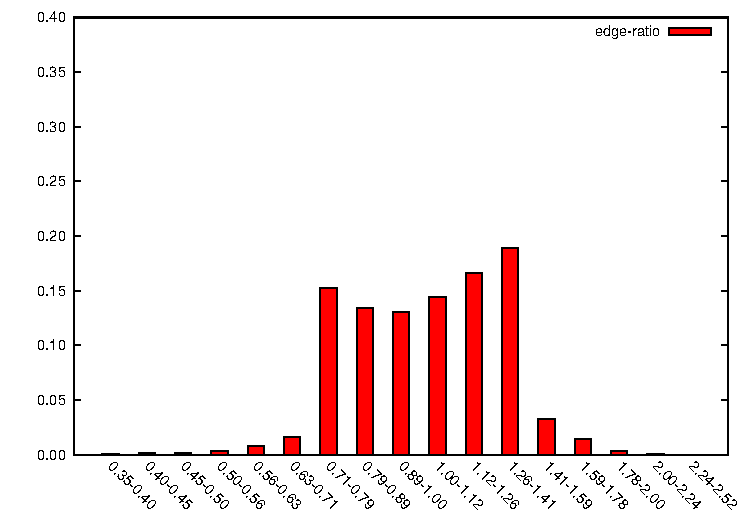
\includegraphics[width=\textwidth]{epic-ic-cube-linear-stats.pdf}
\caption{EPIC-IC}
\end{subfigure}
\begin{subfigure}{.4\textwidth}
\centering
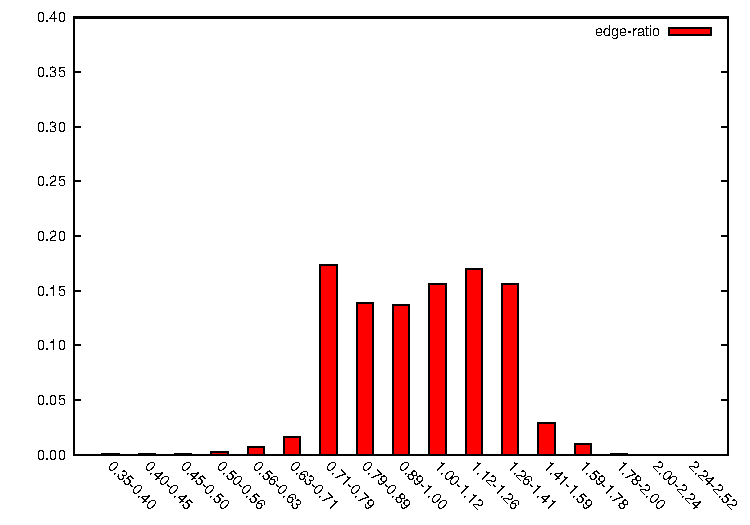
\includegraphics[width=\textwidth]{epic-ics-cube-linear-stats.pdf}
\caption{EPIC-ICS}
\end{subfigure}
\begin{subfigure}{.4\textwidth}
\centering
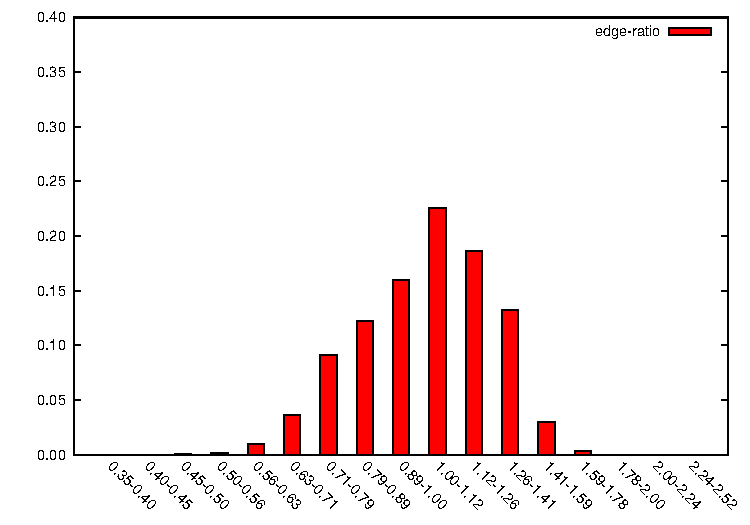
\includegraphics[width=\textwidth]{epic-icsm-cube-linear-stats.pdf}
\caption{EPIC-ICSM}
\end{subfigure}
\begin{subfigure}{.4\textwidth}
\centering
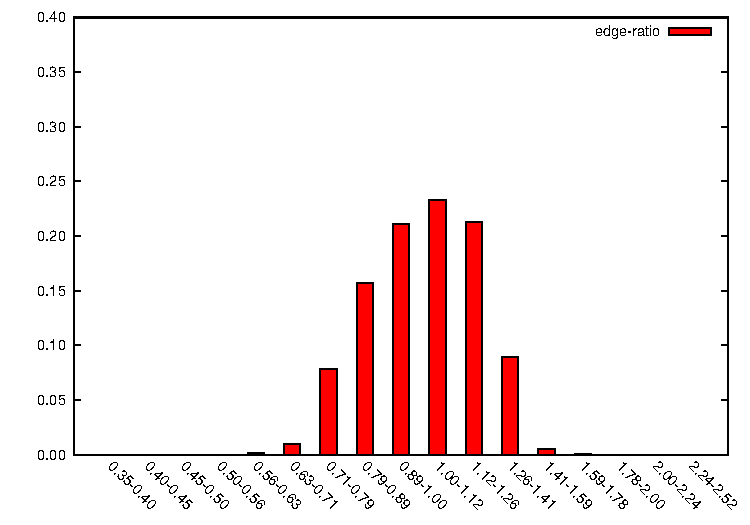
\includegraphics[width=\textwidth]{fefloa-cube-linear-stats.pdf}
\caption{feflo.a}
\end{subfigure}
\begin{subfigure}{.4\textwidth}
\centering
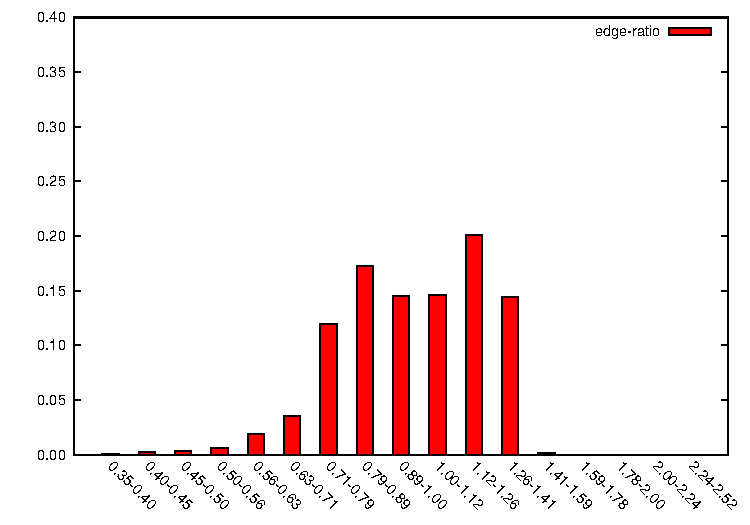
\includegraphics[width=\textwidth]{omega_h-cube-linear-stats.pdf}
\caption{Omega\_h}
\end{subfigure}
\begin{subfigure}{.4\textwidth}
\centering
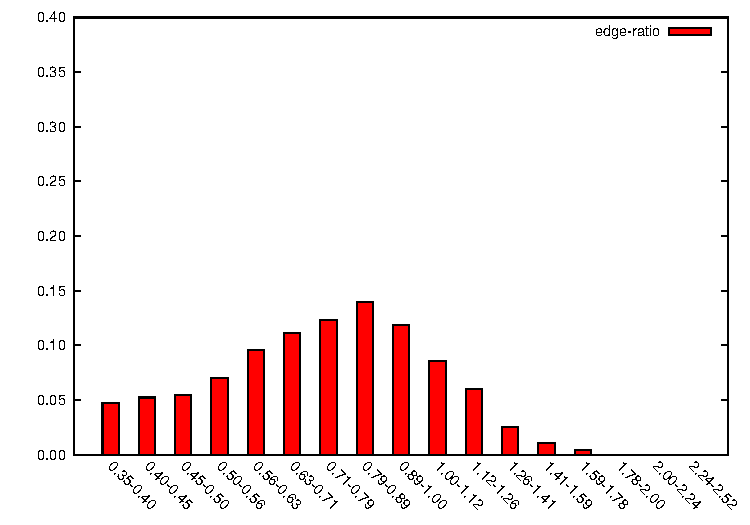
\includegraphics[width=\textwidth]{refine-one-cube-linear-stats.pdf}
\caption{refine/one}
\label{fig:cube-linear-lengths-refine-one}
\end{subfigure}
\begin{subfigure}{.4\textwidth}
\centering
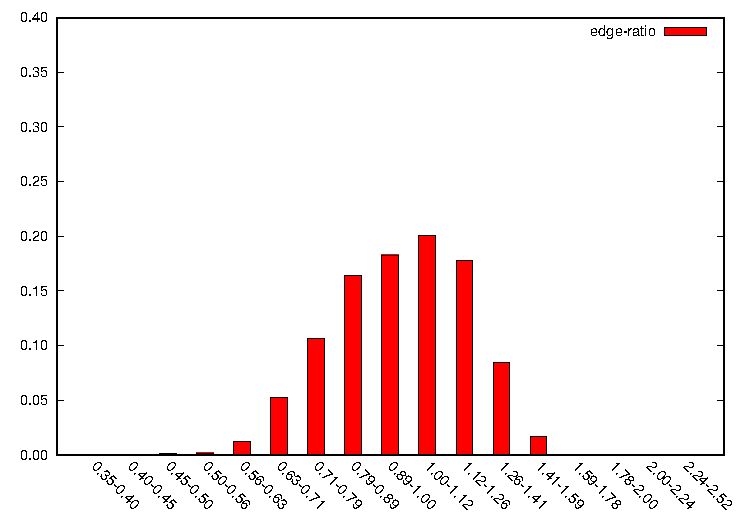
\includegraphics[width=\textwidth]{refine-two-cube-linear-stats.pdf}
\caption{refine/two}
\end{subfigure}
\caption{Length histograms for the linear cube metric}
\label{fig:cube-linear-lengths}
\end{figure}

%\enlargethispage{12pt}

\section{Future Directions}
{\color{red} Adrien}

\section{Conclusion}

\bibliography{references}
\bibliographystyle{model1-num-names}

\end{document}

\clearpage

%%%% This page is for instructions only, once the article is finalize please omit the below text before creating the final PDF
\normalMode

\section*{Instructions to Authors for LaTeX template:}

\section{ZIP mode for LaTeX template:}

The zip package is created as per the guide lines present on the URL http://www.elsevier.com/author-schemas/ preparing-crc-journal-articles-with-latex for creating the LaTeX zip file of Procedia LaTeX template.  The zip generally contains the following files:
\begin{Itemize}[]\leftskip-17.7pt\labelsep3.3pt
\item ecrc.sty
\item  elsarticle.cls
\item elsdoc.pdf
\item .bst file
\item Manuscript templates for use with these bibliographic styles
\item  Generic and journal specific logos, etc.
\end{Itemize}

The LaTeX package is the main LaTeX template. All LaTeX support files are required for LaTeX pdf generation from the LaTeX template package.

{\bf Reference style .bst file used for collaboration support:} In the LaTeX template packages of all Procedia titles a new ``.bst'' file is used which supports collaborations downloaded from the path http://www.elsevier.com/author-schemas/the-elsarticle-latex-document-class

\section{Reference styles used in  Procedia master templates:}
\let\footnotesize\normalsize
\hspace*{-10pt}\begin{tabular*}{\hsize}{@{}ll@{}}
{\bf Title}&{\bf Reference style} \\[6pt]
AASPRO  & 2 Harvard\\
AASRI Procedia  & 3 Vancouver Numbered\\
APCBEE Procedia  & 3 Vancouver Numbered\\
EGYPRO  & 3 Vancouver Numbered\\
FINE    & 2 Harvard\\
IERI Procedia  & 3 Vancouver Numbered\\
MATPR  & 1a Numbered without article titles\\
MSPRO  & 2 Harvard\\
PHPRO  & 2 Harvard\\
PIUTAM  & 3a Embellished Vancouver \\
Procedia CIRP  & 3 Vancouver Numbered\\
PROCHE  & 3a Embellished Vancouver \\
PROCS  & 3a Embellished Vancouver \\
PROENG  & 1 Numbered\\
PROENV  & 3a Embellished Vancouver \\
PROEPS  & 3a Embellished Vancouver \\
PROFOO    & 3a Embellished Vancouver \\
PROMFG  & 1a Numbered without article titles\\
PROTCY  & 3 Vancouver Numbered\\
PROVAC  & 3a Embellished Vancouver \\
SBSPRO  & 5 APA\\
SEPRO  & 3a Embellished Vancouver \\
AQPRO & 2 Harvard\\
UMKPRO & 5 APA\\
\end{tabular*}

\end{document}

%%
%% End of file `procs-template.tex'.
